\documentclass[data-structure.tex]{subfiles}
\begin{document}
%%%%%%%%%%%%%%%%%%%%%%%%%%%%%%%%%%%%%%%%%%%%%%%%%%%%%%%%%%%%%%%%%%%%%%%%%%%%%%%%%%%%%
%%%%%%%%%%%%%   Tree
%%%%%%%%%%%%%%%%%%%%%%%%%%%%%%%%%%%%%%%%%%%%%%%%%%%%%%%%%%%%%%%%%%%%%%%%%%%%%%%%%%%%%%%%%
% \section{Tree}
% \label{concept_tree}
\subsubsection{Terminologies}
A \textbf{tree} is a type of acyclic graph and it is defined as a collection of entities which are called \textbf{nodes}. Nodes are connected by \textbf{edges}. Each node contains a value or data, and it may or may not have a child node. 

The first node of the tree is called the \textbf{root}, if this root node is connected by another node, the root is then a parent node and the connected node is a child node instead. On the other hand, \textbf{leaves} are the last nodes on a tree. They are nodes without children. Just like a real tree, we have the root, branches (substree), and finally the leaves. We can see the root, leave nodes in Fig~\ref{fig:tree_property}.  

A \textbf{path} is defined as a sequence of nodes and edges connecting a node with a descendant.  We can classify them into three types: 
\begin{enumerate}
    \item Root->Leaf Path: the starting and ending node of the path is the root and leaf node respectively;
    \item Root->Any Path: the starting and ending node of the path is the root and any node (Root, inner, leaf node) respectively;
    \item Any->Any Path: the starting and ending node of the path is both any node (Root, inner, leaf node) respectively. 
\end{enumerate}

\subsubsection{Properties}
\begin{figure}[h]
    \centering
    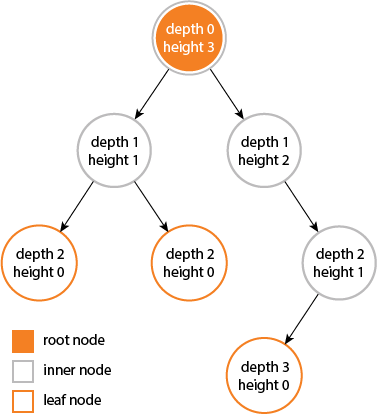
\includegraphics[width=0.6\columnwidth]{fig/tree_property.png}
    \caption{Example of a Tree with height and depth denoted}
    \label{fig:tree_property}
\end{figure}
The property of a tree starts from the property of a \textit{node} (shown in Fig~\ref{fig:tree_property}).
\begin{enumerate}
    \item The \textbf{depth} (or level) of a node is the number of edges from the node to the tree's root node. And it can be obtained from up-down level-by-level traversal.
    \item The \textbf{height} of a node is the number of edges on the \textit{longest path} from the node to a leaf. A leaf node will have a height of 0.
    \item The \textbf{descendant} of a node is any node that is reachable by repeated proceeding from parent to child starting from this node. They are also known as subchild.
    \item The \textbf{ancestor} of a node is any node that is reachable by repeated proceeding from child to parent starting from this node.
    \item The \textbf{degree} of a node is the number of its children. A leaf is necessarily degreed zero. 
\end{enumerate}

Properties of a \textit{tree}:
\begin{enumerate}
    \item The \textbf{height}(or \textbf{depth}) of a tree would be the height of its root node, or equivalently, the depth of its deepest node. 
    \item The \textbf{diameter} (or \textbf{width}) of a tree is the number of nodes (or edges) on the longest path between any two leaf nodes. 
\end{enumerate}

\textbf{Forest} is a set of $n>=0$ disjoint treees. 


\paragraph{Types of Binary Tree}
There are four common types of Binary Tree: 1) Full Binary Tree, 2) Complete Binary Tree, 3) Perfect Binary Tree, 4) Balanced Binary Tree.

\textbf{Full Binary Tree} A binary tree is full if every node has 0 or 2 children. We can also say that a full binary tree is a binary tree in which all nodes except leaves have two children.  In full binary tree, the number of leaves and the number of all other non-leaf nodes has relation: L = Non-L + 1. 

\textbf{Complete Binary Tree} A Binary Tree is complete Binary Tree if all levels are completely filled except possibly the last level and the last level has all keys as left as possible.

\textbf{Perfect Binary Tree} A Binary tree is Perfect Binary Tree in which all internal nodes have two children and all leaves are at the same level.

\textbf{Balanced Binary Tree} A binary tree is balanced if the height of the tree is O(Log n) where n is the number of nodes. For Example, AVL tree maintains O(Log n) height by making sure that the difference between heights of left and right subtrees is 1.

\textbf{A degenerate (or pathological) tree} A Tree where every internal node has one child. Such trees are performance-wise same as linked list.
%%%%%%%%%%%%%%%%%%%%%binary search tree%%%%%%%%%%%%%%%%%%%%%%
\section{Binary Search Tree}
\label{sec_binary_search_tree}
 In computer science, a \textbf{search tree} is a tree data structure used for locating specific keys from within a set. In order for a tree to function as a search tree, the key for each node must be greater than any keys in subtrees on the left and less than any keys in subtrees on the right. 

The advantage of search trees is their efficient search time ( $O(\log n)$) given the tree is reasonably balanced, which is to say the leaves at either end are of comparable depths as we introduced the \textbf{balanced binary tree}. 

The search tree data structure supports many dynamic-set operations, including SEARCH, MINIMUM, MAXIMUM, PREDECESSOR, SUCCESSOR, INSERT, and DELETE. Thus, a search tree can be both used as a dictionary and a priority queue.


% Search trees are often used to implement an associative array. The search tree algorithm uses the key from the key-value pair to find a location, and then the application stores the entire key–value pair at that location. 

In this section, we will introduce the most commonly used two types of searching trees: binary searching tree (BST) and Trie where the keys are usually numeric numbers and strings respectively. 

\subsection{Binary Searching Tree}
\label{concept_binary_search_tree}
A binary search tree (BST) is an organized searching tree structure in binary tree, as the name suggests. Binary search trees whose internal nodes each store a key (and optionally, an associated value), each node have two distinguished sub-trees (if only one sub-tree the other is None). 

BST keep their keys in sorted order, so that lookup and other operations can use the \textit{principle of binary search tree}: 

\indent Let $x$ be a node in a binary search tree, if $y$ is a node in the left subtree of x, them $y.key \leq x.key$. If $y$ is a node in the right subtree of $x$, then $y.key \geq x.key$. 

There are three possible ways to properly define a BST, and we use $l$ and $r$ to represent the left and right child of node $x$: 1)$l.key \leq x.key < r.key$, 2) $l.key  < x.key \leq r.key$, 3) $l.key < x.key < r.key$. In the first and second definition, our resulting BST allows us to have duplicates, while not in the case of the third definiton. One example of BST without duplicates is shown in Fig~\ref{fig:bst}. 
\begin{figure}[h]
    \centering
    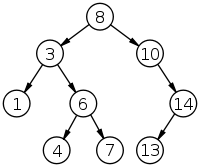
\includegraphics[width = 0.6\columnwidth]{fig/Binary_search_tree.png}
    \caption{Example of Binary search tree of depth 3 and 8 nodes.}
    \label{fig:bst}
\end{figure}

\textbf{Solve Duplicate Problem} When there are duplicates, things can be more complicated, and the college algorithm book did not really tell us what to do when there are duplicates.  If you use the definition "left <= root < right" and you have a tree like:
\begin{lstlisting}[numbers=none]
      3
    /   \
  2       4
\end{lstlisting}

then adding a ``3'' duplicate key to this tree will result in:
\begin{lstlisting} [numbers=none]
      3
    /   \
  2       4
    \
     3
\end{lstlisting}
Note that the duplicates are not in contiguous levels.

This is a big issue when allowing duplicates in a BST representation as the one above: duplicates may be separated by any number of levels, so checking for duplicate's existence is not that simple as just checking for immediate children of a node.

An option to avoid this issue is to not represent duplicates structurally (as separate nodes) but instead use a counter that counts the number of occurrences of the key. The previous example would then have a tree like:
\begin{lstlisting}
      3(1)
    /     \
  2(1)     4(1)
  \end{lstlisting}

and after insertion of the duplicate "3" key it will become:
\begin{lstlisting}
      3(2)
    /     \
  2(1)     4(1)
  \end{lstlisting}

This simplifies SEARCH, DELETE and INSERT operations, at the expense of some extra bytes and counter operations. In the following content, we assume using definition three so that our BST will have no duplicates. 

\subsubsection{Operations}
When looking for a key in a tree (or a place to insert a new key), we traverse the tree from root to leaf, making comparisons to keys stored in the nodes of the tree and deciding, on the basis of the comparison, to continue searching in the left or right subtrees. On average, this means that each comparison allows the operations to skip about half of the tree, so that each SEARCH, INSERT or DELETE takes time proportional to the logarithm of the number of items stored in the tree. This is much better than the linear time required to find items by key in an (unsorted) array, but slower than the corresponding operations on hash tables. 

% \textbf{Definition} A binary search tree is a rooted binary tree, whose internal nodes each store a key (and optionally, an associated value) and each have two distinguished sub-trees, commonly denoted left and right. The tree additionally satisfies the binary search property, which states that the key in each node must be greater than or equal to any key stored in the left sub-tree, and less than or equal to any key stored in the right sub-tree.[1]:287 The leaves (final nodes) of the tree contain no key and have no structure to distinguish them from one another. 

In order to build a BST, we need to INSERT a series of elements in the tree organized by the searching tree property, and in order to INSERT, we need to SEARCH the position to INSERT this element. Thus, we introduce these operations in the order of SEARCH, INSERT and GENERATE. 
\begin{figure}[h]
    \centering
    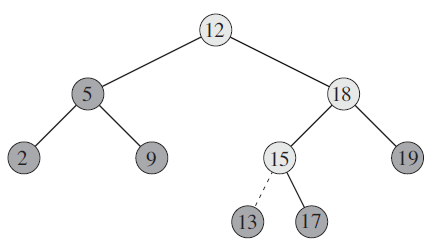
\includegraphics[width=0.6\columnwidth]{fig/bst_insertion.png}
    \caption{The lightly shaded nodes indicate the simple path from the root down to the position where the item is inserted. The dashed line indicates the link in the tree that is added to insert the item. }
    \label{fig:bst_operation}
\end{figure}
\paragraph{SEARCH}

There are two different implementations for SEARCH: recursive and iterative.
\begin{lstlisting}[language = Python]
# recursive searching
def search(root,key):
    # Base Cases: root is null or key is present at root
    if root is None or root.val == key:
        return root
 
    # Key is greater than root's key
    if root.val < key:
        return search(root.right,key)
   
    # Key is smaller than root's key
    return search(root.left,key)
\end{lstlisting}
Also, we can write it in an iterative way, which helps us save the heap space: 
\begin{lstlisting}[language = Python]
# iterative searching
def iterative_search(root,key):
    while root is not None and root.val != key:
        if root.val < key:
            root = root.right
        else:
            root = root.left
    return root
\end{lstlisting}
\paragraph{INSERT}
Assuming we are inserting a node $13$ into the tree shown in Fig~\ref{fig:bst_operation}. A new key is always inserted at leaf (there are other ways to insert but here we only discuss this one way). We start searching a key from root till we hit an empty node. Then we new a TreeNode and insert this new node either as the left or the child node according to the searching property. Here we still shows both the recursive and iterative solutions.
\begin{lstlisting}[language = Python]
# Recursive insertion
def insertion(root, key):
    if root is None:
        root = TreeNode(key)
        return root
    if root.val < key:
        root.right = insertion(root.right, key)
    else:
        root.left = insertion(root.left, key)
    return root
\end{lstlisting}
The above code needs return value and reassign the value for the right and left every time, we can use the following code which might looks more complex with the if condition but works faster and only assign element at the end. 
\begin{lstlisting}[language=Python]
# recursive insertion
def insertion(root, val):
    if root is None:
        root = TreeNode(val)
        return 
    if val > root.val:
        if root.right is None:
            root.right = TreeNode(val)
        else:
            insertion(root.right, val)
    else:
        if root.left is None:
            root.left = TreeNode(val)
        else:
            insertion(root.left, val)
\end{lstlisting}
We can search the node iteratively and save the previous node. The while loop would stop when hit at an empty node.  There will be three cases in the case of the previous node. 
\begin{lstlisting}[numbers=none]
1. The previous node is None, which means the tree is empty, so we assign a root node with the value
2. The previous node has a value larger than the key, means we need to put key as left child.  
3. The previous node has a value smaller than the key, means we need to put key as right child.
\end{lstlisting}
\begin{lstlisting}[language = Python]
# iterative insertion
def iterativeInsertion(root, key):
    pre_node = None
    node = root
    while node is not None:
        pre_node = node
        if key < node.val:
            node = node.left
        else:
            node = node.right
    # we reached to the leaf node which is pre_node
    if pre_node is None:
        root = TreeNode(key)
    elif pre_node.val > key:
        pre_node.left = TreeNode(key)
    else:
        pre_node.right = TreeNode(key)
    return root
\end{lstlisting}
\paragraph{BST Generation}
First, let us declare a node as BST which is the root node. Given a list, we just need to call INSERT for each element. The time complexity can be $O(n\log_n)$.
\begin{lstlisting}[language=Python]
datas = [8, 3, 10, 1, 6, 14, 4, 7, 13]
BST = None
for key in datas:
    BST = iterativeInsertion(BST, key)
print(LevelOrder(BST))
# output 
# [8, 3, 10, 1, 6, 14, 4, 7, 13]
\end{lstlisting}
\paragraph{DELETE} 
Before we start to check the implementation of DELETE, I would suggest the readers to read the next subsection--the Features of BST at first, and then come back here to finish this paragraph. 

When we delete a node, three possibilities arise.
\begin{lstlisting}[numbers=none]
1) Node to be deleted is leaf: Simply remove from the tree.

              50                            50
           /     \         delete(20)      /   \
          30      70       --------->    30     70 
         /  \    /  \                     \    /  \ 
       20   40  60   80                   40  60   80

2) Node to be deleted has only one child: Copy the child to the node and delete the child

              50                            50
           /     \         delete(30)      /   \
          30      70       --------->    40     70 
            \    /  \                          /  \ 
            40  60   80                       60   80

3) Node to be deleted has two children: Find inorder successor of the node. Copy contents of the inorder successor to the node and delete the inorder successor. Note that inorder predecessor can also be used.

              50                            60
           /     \         delete(50)      /   \
          40      70       --------->    40    70 
                 /  \                            \ 
                60   80                           80

The important thing to note is, inorder successor is needed only when right child is not empty. In this particular case, inorder successor can be obtained by finding the minimum value in right child of the node.
\end{lstlisting}
\subsubsection{Features of BST}
\label{concept_features_bst}
\paragraph{Minimum and Maximum} The operation is similar to search, to find the minimum, we always traverse on the left subtree.  For the maximum, we just need to replace the ``left'' with ``right'' in the key word.  Here the time complexity is the same $O(lgn)$.
\begin{lstlisting}[language=Python]
# recursive
def get_minimum(root):
    if root is None:
        return None
    if root.left is None: # a leaf or node has no left subtree
        return root
    if root.left:
        return get_minimum(root.left)

# iterative
def iterative_get_minimum(root):
    while root.left is not None:
        root = root.left
    return root
\end{lstlisting}

Also, sometimes we need to search two additional items related to a given node:  successor and predecessor. The structure of a binary search tree allows us to determine the successor or the predecessor of a tree without ever comparing keys. 

\paragraph{Successor of a Node}  A successor of node $x$ is the smallest item in the BST that is strictly greater than $x$. It is also called in-order successor, which is the next node in Inorder traversal of the Binary Tree. Inoreder Successor is None for the last node in inorder traversal. If our TreeNode data structure has a parent node.

Use parent node: the algorihtm has two cases on the basis of the right subtree of the input node. 
\begin{lstlisting}[numbers=none]
For the right subtree of the node:
1) If it is not None, then the successor is the minimum node in the right subtree. e.g. for node 12, successor(12) = 13 = min(12.right)
2) If it is None, then the successor is one of its ancestors. We traverse up using the parent node until we find a node which is the left child of its parent. Then the parent node here is the successor. e.g.  successor(2)=5
\end{lstlisting}
 The Python code is provided:
\begin{lstlisting}[language = Python]
def Successor(root, n):
# Step 1 of the above algorithm
    if n.right is not None:
        return get_minimum(n.right)
# Step 2 of the above algorithm
p = n.parent
while p is not None:
    if n == p.left :# if current node is the left child node, then we found the successor, p
        return p
    n = p
    p = p.parent
return p
\end{lstlisting}
However, if it happens that your tree node has no parent defined, which means you can not traverse back its parents. We only have one option. Use the inorder tree traversal, and find the element right after the node. \begin{lstlisting}[numbers=none]
For the right subtree of the node:
1) If it is not None, then the successor is the minimum node in the right subtree. e.g. for node 12, successor(12) = 13 = min(12.right)
2) If it is None, then the successor is one of its ancestors. We traverse down from the root till we find current node, the node in advance of current node is the successor. e.g.  successor(2)=5
\end{lstlisting}
\begin{lstlisting}[language=Python]
def SuccessorInorder(root, n):
    # Step 1 of the above algorithm
    if n.right is not None:
        return get_minimum(n.right)
    # Step 2 of the above algorithm
    succ = None
    while root is not None:
        
        if n.val > root.val:
            root = root.right
        elif n.val < root.val:
            succ = root
            root = root.left
        else: # we found the node, no need to traverse
            break
    return succ
\end{lstlisting}

\paragraph{Predecessor of A Node}  A predecessor of node $x$ on the other side, is the largest item in BST that is strictly smaller than $x$. It is also called in-order predecessor, which denotes the previous node in Inorder traversal of BST. e.g. for node 14, predecessor(14)=12= max(14.left). The same searching rule applies, if node $x$'s left subtree exists, we return the maximum value of the left subtree. Otherwise we traverse back its parents, and make sure it is the right subtree, then we return the value of its parent, otherwise the reversal traverse keeps going. 
\begin{lstlisting}[language = Python]
def Predecessor(root, n):
# Step 1 of the above algorithm
    if n.left is not None:
        return get_maximum(n.left)
# Step 2 of the above algorithm
p = n.parent
while p is not None:
    if n == p.right :# if current node is the right node, parent is smaller
        return p
    n = p
    p = p.parent
return p
\end{lstlisting}
 The worst case to find the successor or the predecessor of a BST is to search the height of the tree: include the one of the subtrees of the current node, and go back to all the parents and greatparents of this code, which makes it the height of the tree. The expected time complexity is $O(lgn)$. And the worst is when the tree line up and has no branch, which makes it $O(n)$. 
 
 \paragraph{Lowest Common Ancestor(LCA)} The lowest common ancestor is defined between two nodes v and w as the lowest node in T that has both v and w as descendants (where we allow a node to be a descendant of itself).” e.g., if u=5,w=19, then we first node when we recursively visiting the tree that is within [u,w], then the LCA is 14. Compared with LCA for binary tree, because of the searching property of searching tree, it is even simipler:
 \begin{lstlisting}
 treverse the tree:
  if node.val is in [s, b], return node is LCA
  if node.val > b, traverse node.left
  if node.val < s, traverse node.right
 \end{lstlisting}
 
 235. Lowest Common Ancestor of a Binary Search Tree
 
 Given a binary search tree (BST), find the lowest common ancestor (LCA) of two given nodes in the BST.
\begin{lstlisting}
Given binary search tree:  root = [6,2,8,0,4,7,9,null,null,3,5]

        _______6______
       /              \
    ___2__          ___8__
   /      \        /      \
   0      _4       7       9
         /  \
         3   5

Example 1:

Input: root = [6,2,8,0,4,7,9,null,null,3,5], p = 2, q = 8
Output: 6
Explanation: The LCA of nodes 2 and 8 is 6.

Example 2:

Input: root = [6,2,8,0,4,7,9,null,null,3,5], p = 2, q = 4
Output: 2
Explanation: The LCA of nodes 2 and 4 is 2, since a node can be a descendant of itself 
             according to the LCA definition.
\end{lstlisting}
\begin{lstlisting}[language=Python]
def lowestCommonAncestor(self, root, p, q):
    """
    :type root: TreeNode
    :type p: TreeNode
    :type q: TreeNode
    :rtype: TreeNode
    """
    s = min(p.val,q.val)
    b = max(p.val,q.val)
    def LCA(node):
        if not node:
            return None
        if node.val>b:
            return LCA(node.left)
        if node.val<s:
            return LCA(node.right)
        # current node [s, b], then this is LCA 
        return node
        
    return LCA(root)
\end{lstlisting}
 
In order traverse can be used to sorting. e.g. 230. Kth Smallest Element in a BST
% \item Smallest and the Biggest Value
% \begin{lstlisting}[language = Python]
% #recursive
% def getSmallest(node):
%     if not node:
%          return None
%     if node.left:
%          return getSmallest(node.left)
%     return node
% #iterative        
% def getSmallest(node):
%     while node:
%           node=node.left
%     return node
% \end{lstlisting}
% \end{enumerate}



% \textbf{Insertion and  Generation of BST} Insertion and deletion is not as easy as the operations shown before, because they cause the dynamic set represented by the binary tree to change. Therefore, the data structure must be re-structured to reflect the change in order to keep holding the binary-search-tree property. 

% Insertion is more straightforward, it is a key component to build a BST. To build a BST, we start from an empty root, and we go through a sequence of data that we want to store in BST structure, and insert each one in the right place with the binary search tree property. To insert a node into the BST, at first we search the tree level-by-level starts from the root node, if the value is smaller that the comparing node's key, we move to its left subtree or else to the right subtree till we reach to leaf node. Look at an example, the follwing tree, 

% the code is as follows:

% Thus the code for building a BST is as follows:


% \textcolor{red}{to do: write the whole operations and the definition of BST as a python class}

% DELETE:
% \begin{lstlisting}[language = Python]
% def delete(root,key):
     
%     # Base Cases: root is null or key is present at root
%     if root is None or root.val == key:
%         return root
 
%     # Key is greater than root's key
%     if root.val < key:
%         return search(root.right,key)
   
%     # Key is smaller than root's key
%     return search(root.left,key)
% \end{lstlisting}

Now  we put a table here to summarize the space and time complexity for each operation.
\begin{table}[h]
\begin{small}
\centering
\noindent\captionof{table}{ Time complexity of operations for BST in big O notation }
 \noindent \begin{tabular}{|p{0.33\columnwidth}|p{0.33\columnwidth}| p{0.33\columnwidth}|}
  \hline
 Algorithm & Average & Worst Case  \\ \hline
Space  & $O(n)$& $O(n)$ \\
Search   & $O(lgn)$ & $O(n)$ \\ \hline

Insert & $O(lgn)$ & $O(n)$ \\ 
Delete & $O(lgn)$ & $O(n)$ \\ \hline
\end{tabular}
  \label{tab:msrc_precession}
  \end{small}
\end{table}

% \paragraph{Advanced Features}
% For a BST, the left subtree all have smaller values than the current node, and the right subtree are all bigger than the current node. This concept is useful in trimming BST, see example, $669$. Trim a Binary Search Tree. 


% \section{Augmented Tree}
% According to \textit{Introduction to Algorithms}, augmenting data stuctures are defined as a textbook data structure augmented by storing additional information in it. In this Section, we introduce two types of augmented tree: Trie for pattern matching in static String and Segment Tree for Range Query. 

%https://www.mimuw.edu.pl/~szczurek/TSG2/04_suffix_arrays.pdf

%%%%%%%%%%%%%%Segment Tree%%%%%%%%%%%%%%%
\section{Segment Tree}
\label{sec_segment_tree}
% In this subsection, we discuss another data structure which can efficiently answer dynamic range queries. As a starting point, we discuss a problem of finding the index of the minimum element
% in an array given a range: [i..j]. This is more commonly known as the Range Minimum Query(RMQ). For example, given an array A of size 7 below, RMQ(1, 3) = 2, as the index 2 contains the minimum element among A[1], A[2], and A[3]. To check your understanding of RMQ, verify that on array A below, RMQ(3, 4) = 4, RMQ(0, 0) = 0, RMQ(0, 1) = 1, and RMQ(0, 6) = 5.

% There are several ways to solve this RMQ. One of the trivial algorithm is to simply iterate the
% array from index i to j and report the index with the minimum value. But this is O(n) per query.
% When n is large, such algorithm maybe infeasible.

Segment Tree is a static full binary tree similar to heap that is used for storing the intervals or segments. `Static` here means once the data structure is build, it can not be modified or extended.  Segment tree is a data structure that can efficiently answer numerous \textit{dynamic range queries} problems 
(in logarithmic time) like finding minimum, maximum, sum, greatest common divisor, least common denominator in array. The ``dynamic" means there are constantly modifications of the value of elements (not the tree structure).   For instance, given a problem to find the index of the minimum/maximum/sum of all elements in an given range of an array: [i:j]. 

\paragraph{Definition} Consider an array A of size n and a corresponding Segment Tree T (here a range [0, n-1] in A is represented as A[0:N-1]):
\begin{enumerate}
    \item The root of T represents the whole array A[0:N-1]. 
    \item Each internal node in the Segment Tree T represents the interval of A[i:j] where $0 < i < j < n$. 
    \item Each leaf in T represents a single element A[i], where $0 \leq i<N$. 
    \item If the parent node is in range [i, j], then we separate this range at the middle position $m = (i+j)\/\/2$, the left child takes range [i, m], and the right child take the interval of [m+1, j].
\end{enumerate}

Because in each step of building the segment tree, the interval is divided into two halves, so the height of the segment tree will be $\log N$. And there will be totally N leaves and N-1 number of internal nodes, which makes the total number of nodes in segment tree to be $2N-1$ and make the segment tree a \textit{full binary tree}.

Here, we use the Range Sum Query (RSQ) problem to demonstrate how segment tree works:
\begin{examples}[resume]
\item \textbf{307. Range Sum Query - Mutable (medium).} Given an integer array nums, find the sum of the elements between indices i and j ($i \leq j$), inclusive.The \textit{update(i, val)} function modifies nums by updating the element at index i to val.
\begin{lstlisting}[numbers=none]
Example:

Given nums = [1, 3, 5]

sumRange(0, 2) -> 9
update(1, 2)
sumRange(0, 2) -> 8
\end{lstlisting}
Note:
\begin{enumerate}
    \item 
    The array is only modifiable by the update function.
   \item  You may assume the number of calls to update and sumRange function is distributed evenly.
\end{enumerate}
\paragraph{Solution: Brute-Force.} There are several ways to solve the RSQ. The \textbf{brute-force solution} is to simply iterate the array from index i to j to sum up the elements and return its corresponding index. And it gives $O(n)$ per query, such algorithm maybe infeasible if queries are constantly required.  Because the update and query action distributed evenly, it still gives $O(n)$ time complexity and $O(n)$ in space, which will get LET error. 

\paragraph{Solution: Segment Tree.}  With Segment Tree, we can store the TreeNode's val as the sum of elements in its corresponding interval. We can define a TreeNode as follows:
\begin{lstlisting}[language=Python]
class TreeNode:
    def __init__(self, val, start, end):
        self.val = val
        self.start = start
        self.end = end
        self.left = None
        self.right = None
\end{lstlisting}
As we see in the process, it is actually not necessary if we save the size of the array, we can decide the start and end index of each node on-the-fly and saves space. 
\begin{figure}[h]
    \centering
    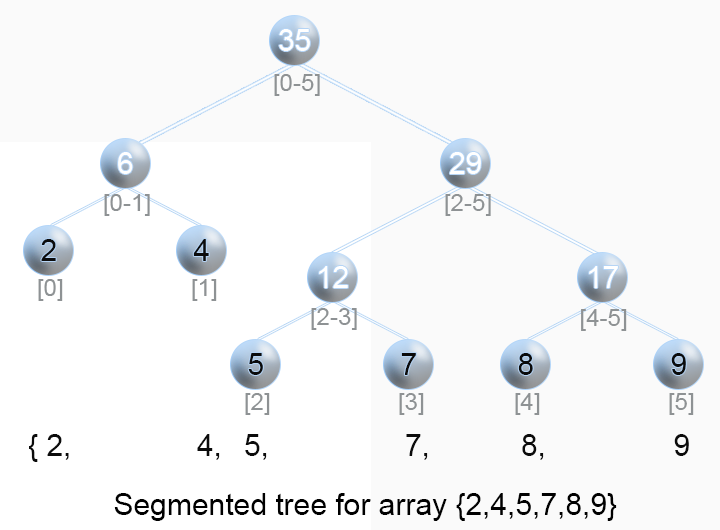
\includegraphics[width=0.8\columnwidth]{fig/307_RSQ_SegmentTree.png}
    \caption{Illustration of Segment Tree. }
    \label{fig:segment_tree}
\end{figure}
\paragraph{Build Segment Tree.} Because the leaves of the tree is a single element, we can use divide and conquer to build the tree recursively.  For a given node, we first build and return its left and right child(including calculating its sum) in advance in the `divide` step, and in the `conquer' step, we calculate this node's sum using its left and right child's sum, and set its left and right child. Because there are totally $2n-1$ nodes, which makes the time and space complexity $O(n)$.
\begin{lstlisting}[language=Python]
def _buildSegmentTree(self, nums, s, e): #start index and end index
    if s > e:
        return None
    if s == e:
        return self.TreeNode(nums[s])
    
    m = (s + e)//2
    # divide 
    left = self._buildSegmentTree(nums, s, m)
    right = self._buildSegmentTree(nums, m+1, e)
    
    # conquer
    node = self.TreeNode(left.val + right.val)
    node.left = left
    node.right = right
    return node
\end{lstlisting}
\paragraph{Update Segment Tree.} Updating the value at index i is like searching the tree for leaf node with range [i, i]. We just need to recalculate the value of the node in the path of the searching. This operation takes $O(\log n)$ time complexity. 
\begin{lstlisting}[language=Python]
def _updateNode(self, i, val, root, s, e):
    if s == e:
        root.val = val
        return 
    m = (s + e)//2
    if i <= m:
        self._updateNode(i, val, root.left, s, m)
    else:
        self._updateNode(i, val, root.right, m+1, e)
    root.val = root.left.val + root.right.val
    return
\end{lstlisting}
\paragraph{Range Sum Query.} Each query range [i, j], will be a combination of ranges of one or multiple ranges. For instance, as in the segment tree  shown in Fig~\ref{fig:segment_tree}, for range [2, 4], it will be combination of [2, 3] and [4, 4]. The process is similar to the updating, we starts from the root, and get its middle index m: 1) if [i, j] is the same as [s, e] that i == s and j == e, then return the value, 2) if the interval [i, j] is within range [s, m] that j <=m , then we just search it in the left branch. 3) if [i, j] in within range [m+1, e] that i>m, then we search for the right branch. 4) else, we search both branch and the left branch has target [i, m], and the right side has target [m+1, j], the return value should be the sum of both sides.  The time complexity is still $O(\log n)$. 
\begin{lstlisting}[language=Python]
def _rangeQuery(self, root, i, j, s, e): 
    if s > e or i > j:
        return 0
    if s == i and j == e:
        return root.val if root is not None else 0
    
    m = (s + e)//2

    if j <= m:
        return self._rangeQuery(root.left, i, j, s, m)
    elif i > m:
        return self._rangeQuery(root.right, i, j, m+1, e)
    else:
        return self._rangeQuery(root.left, i, m, s, m) + self._rangeQuery(root.right, m+1, j, m+1, e)
\end{lstlisting}
The complete code is given: 
\begin{lstlisting}[language=Python]
class NumArray:
    class TreeNode:
        def __init__(self, val):
            self.val = val
            self.left = None
            self.right = None

    def __init__(self, nums):
        self.n = 0
        self.st = None
        if nums:
            self.n = len(nums)
            self.st = self._buildSegmentTree(nums, 0, self.n-1)    
            
    def update(self, i, val):
        self._updateNode(i, val, self.st, 0, self.n -1)       

    def sumRange(self, i, j):
        return self._rangeQuery(self.st, i, j, 0, self.n-1)
\end{lstlisting}
\end{examples}

 

Segment tree can be used here to lower the complexity of each query to $O(log n)$. 

%%%%%%%%%%%%%%%%%%%Trie%%%%%%%%%%%%%%%%%
\section{Trie for String}
\label{concept_trie}
\paragraph{Definition} Trie comes from the word re\textbf{Trie}val. In computer science, a trie, also called digital tree, radix tree or prefix tree which like BST is also a kind of search tree for finding substring in a text. We can solve string matching in $O(|T|)$ time,  where |T| is the size of our text.  This purely algorithmic approach has been studied extensively in the algorithms:  Knuth-Morris-Pratt, Boyer-Moore, and Rabin-Karp. However, we entertain the possibility that multiple queries will be made to the same text.  This motivates the development of data structures that preprocess the text to allow for more efficient queries. Such efficient data structure is Trie, which can do each query in $O(P)$, where P is the length of the pattern string. Trie is an ordered tree structure, which is used mostly for storing strings (like words in dictionary) in a compact way. 
\begin{enumerate}
    \item In a Trie, each child branch is labeled with letters in the alphabet $\sum$. Actually, it is not necessary to store the letter as the key, because if we  order the child branches of every node alphabetically from left to right, the position in the tree defines the key which it is associated to. 
    \item The root node in a Trie represents an empty string. 
\end{enumerate}
% An ordered tree data structure used to store a dynamic set or associative array where the keys are usually strings. Unlike a binary search tree, no node in the tree stores the key associated with that node; instead, its position in the tree defines the key with which it is associated. 

Now, we define a trie Node: first it would have a bool variable to denote if it is the end of the word and a children which is a list of of 26 children TrieNodes. 
\begin{lstlisting}[language= Python]
class TrieNode:
    # Trie node class
    def __init__(self):
        self.children = [None]*26
        # isEndOfWord is True if node represent the end of the word
        self.isEndOfWord = False
\end{lstlisting}
\begin{figure}[h]
    \centering
    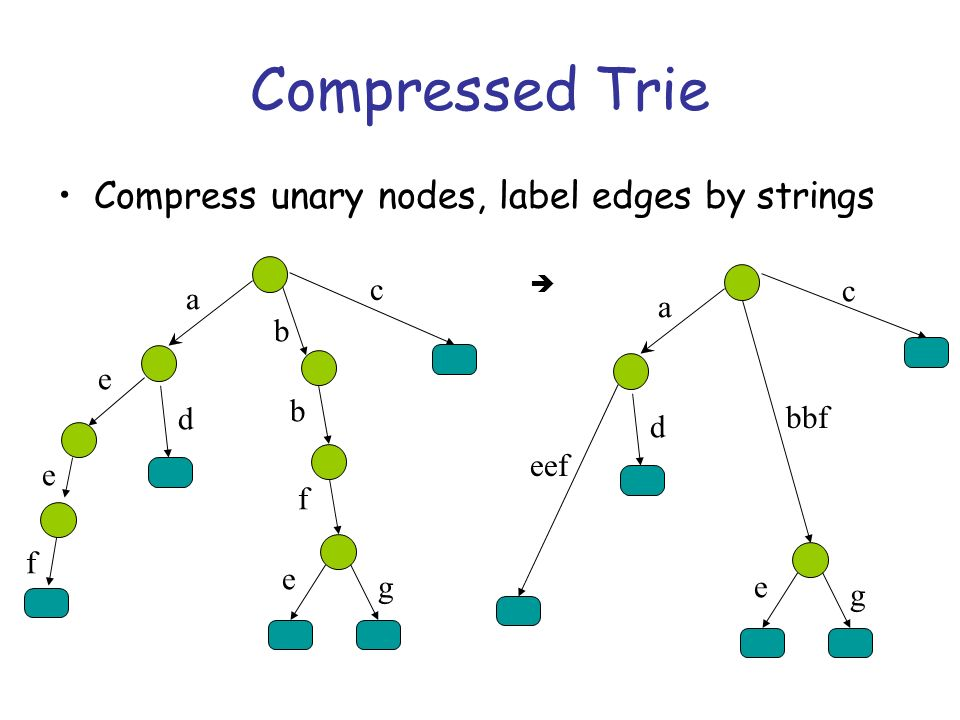
\includegraphics[width=0.6\columnwidth]{fig/trie_compact_trie.jpg}
    \caption{Trie VS Compact Trie}
    \label{fig:trie_compact_trie}
\end{figure}

\paragraph{Compact Trie} If we assign only one letter per edge, we are not taking full advantage of the trie’s tree structure. It is more useful to consider compact or compressed tries, tries where we remove the one letter per edge constraint, and contract non-branching paths by concatenating the letters on these paths.
In this way, every node branches out, and every node traversed represents a choice between two different words.  The compressed trie that corresponds to our example trie is also shown in Figure
~\ref{fig:trie_compact_trie}. 

\paragraph{Operations: INSERT, SEARCH}
% Now, let us solve an LeetCode problem together which requires us to implement a complete Trie that with the operations INSERT, SEARCH, STARTWITH. All of these operations are actually quickly similar and they all require us to simultaneously iterate each character in the input string (or word) and each level of the Trie on the location of that character. So, it would not be hard to get the worst time complexity when we searched the whole tree or finished iterating the characters in the input. 
Both for INSERT and SEARCH, it takes $O(m)$, where m is the length of the word/string we wand to insert or search in the trie. Here, we use an LeetCode problem as an example showing how to implement INSERT and SEARCH. Because constructing a trie is a series of INSERT operations which will take $O(n*m)$, n is the total numbers of words/strings, and m is the average length of each item. The space complexity fof the non-compact Trie would be $O(N*|\sum|)$, where $|\sum|$ is the alphlbetical size, and N is the total number of nodes in the trie structure. The upper bound of N is $n*m$. 
\begin{figure}[h]
    \centering
    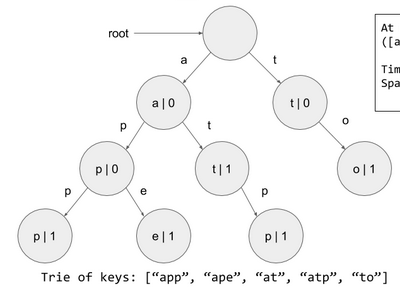
\includegraphics[width=0.6\columnwidth]{fig/Trie.png}
    \caption{Trie Structure}
    \label{fig:trie}
\end{figure}
\begin{examples}
\item \textbf{208. Implement Trie (Prefix Tree) (medium).} Implement a trie with insert, search, and startsWith methods.
\begin{lstlisting}
Example:
Trie trie = new Trie();
trie.insert("apple");
trie.search("apple");   // returns true
trie.search("app");     // returns false
trie.startsWith("app"); // returns true
trie.insert("app");   
trie.search("app");     // returns true
\end{lstlisting}
\textit{Note: You may assume that all inputs are consist of lowercase letters a-z. All inputs are guaranteed to be non-empty strings.}

\paragraph{INSERT} with INSERT operation, we woould be able to insert a given word in the trie, when traversing the trie from the root node which is a TrieNode, with each letter in world, if its corresponding node is None, we need to put a node, and continue. At the end, we need to set that node's endofWord variable to True. thereafter, we would have a new branch starts from that node constructured. For example, when we first insert ``app`` as shown in Fig~\ref{fig:trie_compact_trie}, we would end up building branch ``app``, and with ape, we would add nodes ``e`` as demonstrated with red arrows. 
\begin{lstlisting}[language=Python]
def insert(self, word):
    """
    Inserts a word into the trie.
    :type word: str
    :rtype: void
    """
    node = self.root #start from the root node
    for c in word:
        loc = ord(c)-ord('a')
        if node.children[loc] is  None: # char does not exist, new one
            node.children[loc] = self.TrieNode()
        # move to the next node
        node = node.children[loc]
    # set the flag to true
    node.is_word = True 
\end{lstlisting}

\paragraph{SEARCH} For SEARCH, like INSERT, we traverse the trie using the letters as pointers to the next branch. There are three cases: 1) for word P, if it doesnt exist, but its prefix does exist, then we return False. 2) If we found a matching for all the letters of P, at the last node, we need to check if it is a leaf node where is\_word is True.  STARTWITH is just slightly different from SEARCH, it does not need to check that and return True after all letters matched. 
\begin{lstlisting}[language=Python]
def search(self, word):
    node = self.root
    for c in word:
        loc = ord(c)-ord('a')
        # case 1: not all letters matched 
        if node.children[loc] is None: 
            return False          
        node = node.children[loc]
    # case 2
    return True if node.is_word else False
\end{lstlisting}
\begin{lstlisting}[language=Python]
def startWith(self, word):
    node = self.root
    for c in word:
        loc = ord(c)-ord('a')
        # case 1: not all letters matched 
        if node.children[loc] is None: 
            return False          
        node = node.children[loc]
    # case 2
    return True
\end{lstlisting}
Now complete the given Trie class with TrieNode and \_\_init\_\_ function.
\begin{lstlisting}[language=Python]
class Trie:
    class TrieNode:
        def __init__(self):
            self.is_word = False
            self.children = [None] * 26 #the order of the node represents a char

    def __init__(self):
        """
        Initialize your data structure here.
        """
        self.root = self.TrieNode() # root has value None       
\end{lstlisting}
\end{examples}

\begin{examples}
\item \textbf{336. Palindrome Pairs (hard).} Given a list of unique words, find all pairs of distinct indices (i, j) in the given list, so that the concatenation of the two words, i.e. words[i] + words[j] is a palindrome.
\begin{lstlisting}
Example 1:

Input: ["abcd","dcba","lls","s","sssll"]
Output: [[0,1],[1,0],[3,2],[2,4]] 
Explanation: The palindromes are ["dcbaabcd","abcddcba","slls","llssssll"]

Example 2:

Input: ["bat","tab","cat"]
Output: [[0,1],[1,0]] 
Explanation: The palindromes are ["battab","tabbat"]
\end{lstlisting}
\textbf{Solution: One Forward Trie and Another Backward Trie.}  We start from the naive solution, which means for each element, we check if it is palindrome with all the other strings. And from the example 1, [3,3] can be a pair, but it is not one of the outputs, which means this is a combination problem, the time complexity is ${C_n}{C_{n-1}}$, and multiply it with the average length of all the strings, we make it $m$, which makes the complexity to be $O(mn^2)$. However, we can use Trie Structure, 
\begin{lstlisting}[language = Python]
from collections import defaultdict


class Trie:
    def __init__(self):
        self.links = defaultdict(self.__class__)
        self.index = None
        # holds indices which contain this prefix and whose remainder is a palindrome
        self.pali_indices = set()

    def insert(self, word, i):
        trie = self
        for j, ch in enumerate(word):
            trie = trie.links[ch]
            if word[j+1:] and is_palindrome(word[j+1:]):
                trie.pali_indices.add(i)
        trie.index = i


def is_palindrome(word):
    i, j = 0, len(word) - 1
    while i <= j:
        if word[i] != word[j]:
            return False
        i += 1
        j -= 1
    return True


class Solution:
    def palindromePairs(self, words):
        '''Find pairs of palindromes in O(n*k^2) time and O(n*k) space.'''
        root = Trie()
        res = []
        for i, word in enumerate(words):
            if not word:
                continue
            root.insert(word[::-1], i)
        for i, word in enumerate(words):
            if not word:
                continue
            trie = root
            for j, ch in enumerate(word):
                if ch not in trie.links:
                    break
                trie = trie.links[ch]
                if is_palindrome(word[j+1:]) and trie.index is not None and trie.index != i:
                    # if this word completes to a palindrome and the prefix is a word, complete it
                    res.append([i, trie.index])
            else:
                # this word is a reverse suffix of other words, combine with those that complete to a palindrome
                for pali_index in trie.pali_indices:
                    if i != pali_index:
                        res.append([i, pali_index])
        if '' in words:
            j = words.index('')
            for i, word in enumerate(words):
                if i != j and is_palindrome(word):
                    res.append([i, j])
                    res.append([j, i])
        return res
\end{lstlisting}
\textbf{Solution2: .}Moreover, there are always more clever ways to solve these problems. Let us look at a clever way:
 abcd, the prefix is ''. 'a', 'ab', 'abc', 'abcd', if the prefix is a palindrome, so the reverse[abcd], reverse[dc], to find them in the words, the words stored in the words with index is fastest to find. $O(n)$. Note that when considering suffixes, we explicitly leave out the empty string to avoid counting duplicates. That is, if a palindrome can be created by appending an entire other word to the current word, then we will already consider such a palindrome when considering the empty string as prefix for the other word.
 \begin{lstlisting}[language = Python]
 class Solution(object):
    def palindromePairs(self, words):
        # 0 means the word is not reversed, 1 means the word is reversed
        words, length, result = sorted([(w, 0, i, len(w)) for i, w in enumerate(words)] +
                                   [(w[::-1], 1, i, len(w)) for i, w in enumerate(words)]), len(words) * 2, []

        #after the sorting,the same string were nearby, one is 0 and one is 1
        for i, (word1, rev1, ind1, len1) in enumerate(words):
            for j in xrange(i + 1, length):
                word2, rev2, ind2, _ = words[j]
                #print word1, word2
                if word2.startswith(word1): # word2 might be longer 
                    if ind1 != ind2 and rev1 ^ rev2: # one is reversed one is not
                        rest = word2[len1:]
                        if rest == rest[::-1]: result += ([ind1, ind2],) if rev2 else ([ind2, ind1],) # if rev2 is reversed, the from ind1 to ind2
                else:
                    break # from the point of view, break is powerful, this way, we only deal with possible reversed, 
        return result
 \end{lstlisting}
 \end{examples}
 
 %https://fizzbuzzed.com/top-interview-questions-5/
% \paragraph{Searching}
% \paragraph{Insertion}
% \paragraph{Deletion}

% Let us see the complete code of a Trie Class:
% \begin{lstlisting}[language = Python]
 
% class Trie:
     
%     # Trie data structure class
%     def __init__(self):
%         self.root = self.getNode()
 
%     def getNode(self):
     
%         # Returns new trie node (initialized to NULLs)
%         return TrieNode()
 
%     def _charToIndex(self,ch):
         
%         # private helper function
%         # Converts key current character into index
%         # use only 'a' through 'z' and lower case
         
%         return ord(ch)-ord('a')
 
 
%     def insert(self,key):
         
%         # If not present, inserts key into trie
%         # If the key is prefix of trie node, 
%         # just marks leaf node
%         pCrawl = self.root
%         length = len(key)
%         for level in range(length):
%             index = self._charToIndex(key[level])
 
%             # if current character is not present
%             if not pCrawl.children[index]:
%                 pCrawl.children[index] = self.getNode()
%             pCrawl = pCrawl.children[index]
 
%         # mark last node as leaf
%         pCrawl.isEndOfWord = True
 
%     def search(self, key):
         
%         # Search key in the trie
%         # Returns true if key presents 
%         # in trie, else false
%         pCrawl = self.root
%         length = len(key)
%         for level in range(length):
%             index = self._charToIndex(key[level])
%             if not pCrawl.children[index]:
%                 return False
%             pCrawl = pCrawl.children[index]
 
%         return pCrawl != None and pCrawl.isEndOfWord
 
% # driver function
% def main():
 
%     # Input keys (use only 'a' through 'z' and lower case)
%     keys = ["the","a","there","anaswe","any",
%             "by","their"]
%     output = ["Not present in trie",
%               "Present in tire"]
 
%     # Trie object
%     t = Trie()
 
%     # Construct trie
%     for key in keys:
%         t.insert(key)
 
%     # Search for different keys
%     print("{} ---- {}".format("the",output[t.search("the")]))
%     print("{} ---- {}".format("these",output[t.search("these")]))
%     print("{} ---- {}".format("their",output[t.search("their")]))
%     print("{} ---- {}".format("thaw",output[t.search("thaw")]))
 
% if __name__ == '__main__':
%     main()
% \end{lstlisting}
There are several other data structures, like balanced trees and hash tables, which give us the possibility to search for a word in a dataset of strings. Then why do we need trie? Although hash table has $O(1)$ time complexity for looking for a key, it is not efficient in the following operations :
\begin{itemize}
    \item Finding all keys with a common prefix.
    \item Enumerating a dataset of strings in lexicographical order.
\end{itemize}

\paragraph{Sorting}
Lexicographic sorting of a set of keys can be accomplished by building a trie from them, and traversing it in pre-order, printing only the leaves' values. This algorithm is a form of radix sort. This is why it is also called radix tree. 

% \paragraph{Dynamic Programming for Static Array}



\end{document}